\documentclass[MScCS]{uccthesis}

\title{Rational Bloom Filters}
\author{Ross Heaney}
\supervisor{Dr Marc Van Dongen}
\secondreader{Dr Who}
\date{\today}

\newcommand*{\COMMAND}[1]{\texttt{\textbackslash #1}}
\newcommand*{\COMMANDWITHARGUMENT}[2]{\texttt{\textbackslash #1}\{#2\}}

\addbibresource{mybib.bib}% should be in preamble

\abstract{%
Bloom Filters are a type of space-efficient probabilistic data structure that can be used to test whether an element is a member of a set. That is when the Bloom Filter is queried 'does this element exist in the set?' and the Bloom Filter returns 'yes' when in fact the element does not exist in the set. We accept these false positives as by agreeing to occasionally get a false positive, we gain an enormous space advantage versus had we refused to accept a false positive.  Using mathematics we can know in advance our false positive rate and tune the bloom filter accordingly. Namely, by setting the size of our bit array to $\frac{K}{S}\ln(2)$ we can reduce the false positive rate of the bloom filter to $2^{-K}$, which is optimal. Given a maximum, allowed false positive rate, r, finding the optimal (minimal) value for k is easy. By assumption k is integral, which makes it difficult to tune a Bloom filter when the desired false positive rate is almost of the form $2^{-k}$. For example, a small change in r may result in a significant increase in the size of the filter, especially when k is small. This thesis is about relaxing this integrality assumption and comparing to the state of the art.
}

%\dedication{%
%   Your dedication here.
%}

%\acknowledgement{%
%   Your acknowledgement here.
%}

\renewcommand\addToFrontMatter[0]{%
}

\begin{document}
\chapter{Introduction}

Bloom Filters are a type of space-efficient probabilistic data structure that can be used to test whether an element is a member of a set. They have exploded in popularity as their usefulness is proportional to the size of the membership set. That is, the larger the size of the dataset we wish to query, the more useful Bloom Filters are. With ever-increasing amounts of data being produced and pipelined year after year, the more Bloom Filters have become almost necessary. In this first chapter I will discuss my thesis mission and the literature review plan. I then follow on with the background and related work in chapter 2. Specifically I discuss the origins of the Bloom Filter via the original paper by Bloom\cite{bloom1970space} and discuss important mathematical results by Kirsch and Mitzenmacher as well as a small but important detail from the book by Mitzenmacher and Upfal\cite{kirsch2006less}\cite{mitzenmacher2017probability}.

\section{Motivations}
As mentioned in the Introduction, bloom filters are a type space efficient probabilistic data structure. First conceived in the 1970s, Bloom Filters have seen widespread use ever since. Today they are used in a variety of applications, including network security, distributed systems, and databases. As data gets larger and larger it becomes more and more difficult to store and process it. Bloom Filters are a way to store and process data in a space efficient manner. This is done by using the so called 'Allowable Error Hashing' technique proposed in the landmark paper, by Burton Howard Bloom, in 1970\cite{bloom1970space}. This technique allows for a trade-off between the space efficiency and the accuracy of the data structure. More importantly, we can tune and optimize the Bloom Filter in relation to the accuracy and space efficiency of the data structure. Specifically this project and thesis titled 'Rational Bloom Filters' will focus on looking at new ways to tune and optimize the Bloom Filter with a specific focus on relaxing the integrality assumption of the number of hash functions required for the Bloom Filter to function properly.

\section{Thesis Mission}
Bloom Filters are based on hashing. Specifically hashing where we accept there will be some hash collisions that will give rise to so called 'false positives'. That is when the Bloom Filter is queried 'does this element exist in the set?' and the Bloom Filter returns 'yes' when in fact the element does not exist in the set. We accept these false positives as by agreeing to occasionally get a false positive, we gain an enormous space advantage versus had we refused to accept a false positive.  Using mathematics we can know in advance our false positive rate and tune the bloom filter accordingly. Namely, by setting the size of our bit array to $\frac{K}{S}\ln(2)$ we can reduce the false positive rate of the bloom filter to $2^{-K}$, which is optimal. Given a maximum, allowed false positive rate, r, finding the optimal (minimal) value for k is easy. By assumption k is integral, which makes it difficult to tune a Bloom filter when the desired false positive rate is almost of the form $2^{-k}$. For example, a small change in r may result in a significant increase in the size of the filter, especially when k is small. This thesis is about relaxing this integrality assumption and comparing to the state of the art.

\chapter{Background and Literature Review}
In this chapter I will discuss the background and related work in the area of bloom filters. Specifically I will discuss the concept of a bloom filter before discussing the original paper by Bloom and the recent work done on bloom filters as it relates to this thesis. Throughout, I will be discussing important mathematical results that are relevant to the thesis.
\section{Concept of a Bloom Filter}
The concept of a bloom filter is summarized nicely in this diagram \ref{fig:bloomfilter}. The core idea behind bloom filters is the concept of hashing. Hashing is simply the transformation of an input value to an output value. In a bloom filter, sometimes a different input will transform to the same output. This is called a hash collision. In certain use cases such as cryptography, hash collisons can be very dangerous, but in the case of Bloom Filters, we accept hash collisions. So, naturally the question is why do we allow hash collisons in Bloom Filters? The answer to that question is space efficiency. By allowing hash collisions we can reduce the space required to store the data structure. This will be discussed in more detail in the next section. For now, it is important to note that the core idea behind a bloom filter is the concept of hashing and allowing hash collisions. The core use case of a Bloom Filter is testing set membership. This is where we can query whether 'x' is present in the Bloom Filter or not. The Bloom Filter will respond either "possibly in the set" or "definitely not in the set". The Bloom Filter will never return a \textit{false negative} but \textit{false positives} are possible.

\begin{figure}[h]
    \centering
    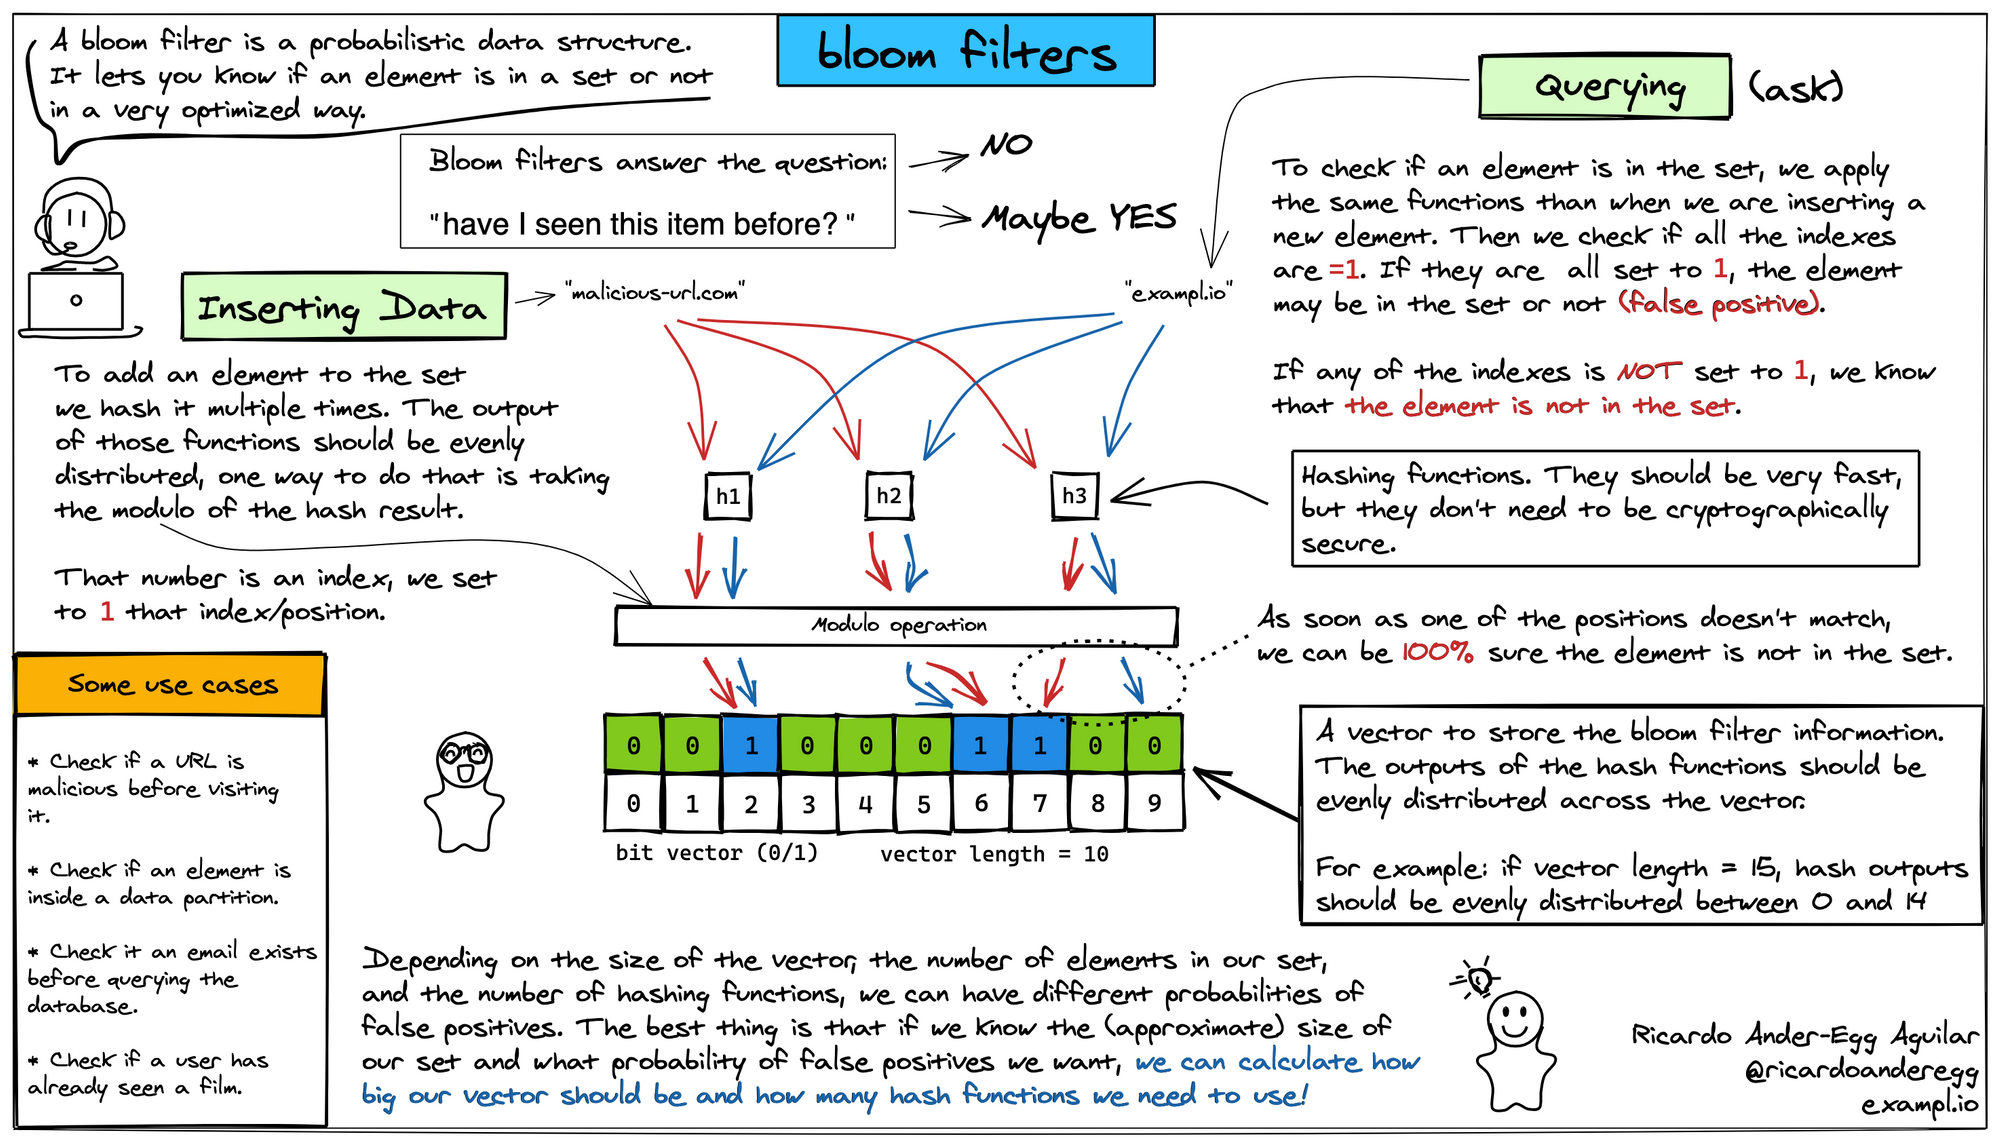
\includegraphics[width=\linewidth]{figures/bloom-filters-poster.png}
    \caption{Bloom Filter Summary}
    \label{fig:bloomfilter}
\end{figure}

\begin{figure}[h]
    \centering
    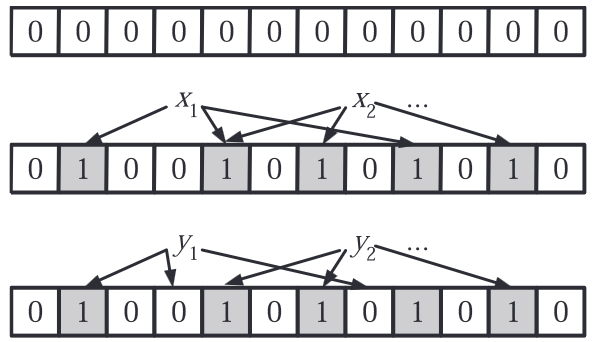
\includegraphics[width=\linewidth]{figures/bloom_filter_example.png}
    \caption{An example of a bloom filter taken from \cite{broder2004network}.The filter begins as an array of all 0s. Each item in the set xi is hashed k times, with each hash yielding a bit location; these bits are set to 1. To check if an element y is in the set, hash it k times and check the corresponding bits. The element y1 cannot be in the set, since a0 is found at one of the bits. The element y2 is either in the set or the filter has yielded a false positive.}
    \label{fig:bloomfilterExample}
\end{figure}



\section{Original Paper by Burton Howard Bloom}
The paper was the first paper to introduce the idea of \textit{Allowable Error Hashing}, which is the basis of Bloom Filters. The essence of Bloom Filters is that set membership, is this item in this set?, can be answered in one of two ways. The first way is to return \underline{yes this item is in the set} and the other way is to say \underline{no this item is not in the set}. Bloom Filters \textbf{guarantee} that false negatives are not possible, while occasionally a false positive is possible. In other words when a Bloom Filter is queried whether an item is in the set or not, it will return "possibly in the set" or "definitely not in the set". The underlying mechanism for the construction of a Bloom Filter is a number of hash functions that map elements of a set to indices on an array. This can be seen in Figure \ref{fig:bloomfilter}. The paper introduced the key concept of an \textit{Allowable Error Rate}. By accepting that we will get a false positive occasionally, we can achieve remarkable space efficiency. The paper's proposed idea is analysed quite nicely via a mathematical comparison between the conventional error-free hashing, state of the art in the 1970s, and the authors proposed \textit{Allowable Error Hashing}. It should be noted that some errors have been found in the original paper and updates published\cite{bose2008false}. The errors found are mostly to do with edge cases and do not necessarily diminish the original paper's contribution. The paper discusses an example of a hyphenation algorithm. Suppose we have a dictionary of 500,000 words of which 90\% follow simple hyphenation rules but the remaining 10\% require expensive disk access to retrieve very specific hyphenation rules that are stored on the disk. By applying the authors \textit{Allowable Error Hashing} technique, disk access is greatly reduced. A hash area only 15\% of the total size needed by an error-free hash cuts down on 85\% of the disk access required. The main idea is not that error-free hashing is bad but rather there is a proposed alternative called \textit{Allowable Error Hashing} that is better suited to certain applications.

\section{Less Hashing, Same Performance}
he paper by  Kirsch and Mitzenmacher \cite{kirsch2006less} is a very nice paper that discusses the number of necessary hash functions to implement a Bloom Filter without any loss in asymptotic false positive probability. Specifically the paper proves a mathematical result that only two hash functions are necessary to implement the Bloom Filter. This paper is \textbf{not} saying that only two hash functions are all that is required for all Bloom Filters, rather that in certain cases only two hash functions are required. This is a vitally important result as it means we can limit our computation overhead and maintain the same performance. Bloom filters are randomized data structures as they rely on pseudorandom hash functions. By reducing the number of hash functions needed then this cuts down on much of the non-trivial computation required to create a Bloom Filter. The important result that was proved in this paper is the following mathematical statement: $(1-e^\frac{-kn}{m})^k$, where m is array size in bits, n is the number of elements in the m size array and k is the number of hash functions. This formula gives us the approximate probability of false positives but Mitzenmacher did it without the assumption of independence, an important distinction from previous mathematical analysis done in other papers. Also related, The book by Mitzenmacher and Upfal \cite{mitzenmacher2017probability} is a very nice book on probability and computing that discusses Bloom Filters in a dedicated subchapter. The important takeaway from the chapter among many other things is that the if you have an m-bit Bloom filter with n elements inserted, then the optimal number k of hash functions to use is $k = \frac{m}{n}\ln 2$.

\section{Network Applications of Bloom Filters}
This survey paper\cite{broder2004network} discusses some very interesting applications for Bloom Filters and essential bloom filter background information. It's an important paper to get a better understanding of Bloom Filters and their uses. Specifically it discusses four instances of network related applications for Bloom Filters and their backgrounds as it relates to the use of Bloom filters. The four instances are as follows:
\begin{itemize}
    \item Collaborating in overlay and peer-to-peer networks
    \item Resource routing
    \item Packet routing
    \item Network measurement
\end{itemize}
I found the network measurement application to be the most interesting application of the four. Essentially the use of Bloom filters for the network measurement problem revolves around the fact that Bloom filters can help us to answer difficult questions about the network. How many packets from a given flow pass through a router? Has a packet from this source passed through a router recently? Bloom filters have proven to be very useful in answering these questions. Whilst not strictly related to this thesis as this thesis is about relaxing the integrality assumption of $k$, it was enlightening to see different use cases of Bloom filters that I had not considered before.

The survey paper also reviews important mathematical background surrounding Bloom filters. Assuming hash functions are perfectly random, the false positive rate(FPR) can be estimated as follows, after all the elements of set $S$ are hashed into the bloom filter, the probability that a specific bit is still 0 is

$ p ' = (1 - \frac{1}{m})^{kn} \approx e ^{-kn/m}$.

Subsequently, if we let $p = e ^{-kn/m}$ a decent approximate and now let p be the proportion of 0 bits after all the $n$ elements are inserted in the bloom filter, then the probability of a false positive is $(1-p)^k \approx (1-p')^k \approx (1-p)^k$.

The total number of bits in the filter is still $m$ and the number of hash functions is still $k$. The probability that a specific bit in the filter is 0 is still $(1-\frac{k}{m})^n \approx e^{-kn/m}$.

Perhaps the most interesting section of the paper, in my opinion is the section on standard Bloom filter tricks. Specifically mathematical tricks. For example, suppose that two Bloom filters represent sets $S_1$ and $S_2$, both with the same number of bits and using the exact same hash functions. Then a Bloom filter that represents the union of the two sets can be obtained by taking the OR($\lor$) of the two bit vectors of the original Bloom filters. Also, another interesting idea is that Bloom filters can be easily halved in size which allows for the dynamic shrinking of a Bloom filter. Suppose the size of the Bloom filter is a power of 2. In order to halve the size of the Bloom filter we would just OR($\lor$) the first and second halves together and then when hashing is performed to query is an element in the set? The highest order bit can be masked, thus preserving the performance.

These are just some interesting mathematical tricks that are discussed in the paper.


\section{Probability and Computing by Mitzenmacher and Upfal}
As we have already established, Bloom filters rely entirely on hashing. A subchapter in the book by Mitzenmacher and Upfal \cite{mitzenmacher2017probability} titled 'Hashing' discusses various hashing techniques. For this thesis, the section dedicated to Bloom filters is of great interest. It discusses important hashing background for Bloom filters. Specifically the following two topics
\begin{itemize}
    \item Chain Hashing
    \item Hashing Bit Strings
\end{itemize}
A useful mental model to have when thinking of chain hashing is the balls-and-bins model. We have $m$ balls that are thrown into $n$ bins, with the location of each ball chosen independently and uniformly at random from the $n$ possibilities. The key question is \textit{What does the distribution of the balls in the bins look like?}. We can also ask \textit{how many of the bins are empty?}, \textit{How many balls are in the fullest bin?}. These questions and their answers are outside the scope of this thesis, but they have many relevant applications to the design and analysis of algorithms. For this thesis the balls-and-bins model serves as a useful mental model to generate insight into Chain hashing and Hashing bit strings. For example suppose we have a password checker application that checks if a password is in a database of passwords in order to prevent users from using bad passwords. When a user signs up for our application we would like to see if the password is part of the 'acceptable' set or the 'unacceptable' set.  One possible approach would be to store the unacceptable passwords(Note for sake of simplicity we are ignoring best security practices regarding passwords)alphabetically and then do a binary search on the set to check if a proposed password is unacceptable. This approach would require $\varTheta (\log m )$ time for $m$ words. Another possibility is to place the unacceptable passwords into bins and then search the appropriate bin for the password. This could be done via a linked list. The placement of the passwords into the bins would be done via hash functions. Essentially a hash function $f$ maps from a universal set $U$ into a range $[0, n - 1]$. This is just a fancy way of saving the hash function will distribute our passwords across a set of bins.

Of course the assumption is that the hash function is well designed and distributes at random. The theory behind these well designed hash functions is outside the scope of this thesis. However for our case the assumption that the hash function distributes at random is a fair one. More rigoursly we assume that (a) for each $x \in U$, the probability  that $f(x)= j$ is $ 1 / n  (for 0 \leq j \leq n -1)$ and that values of $f(x)$ for each $x$ are independent of each other. This does not mean that every output of $f(x)$ is a different random answer, rather it is just equally likely to take on any value in the range. For searching we say there are $n$ bins and $m$ passwords. To search for an item, we first hash it to find the bin that it lies in and then search sequentially through
the linked list for it. If it's not present in our dictionary then the expected number of passwords in the bin the password hashes to is $m/n$. If it is in the dictionary the expected number of passwords in the bin is $1 + (m - 1)/n$. If we chose $n = m$ bins for our hash table, then the number of passwords we must search through in a bin is constant.

In the worse case scenario, the maximum time to search for a word is proportional to the maximum number of words in the bin. When $n = m $ this is $ \vartheta(\ln n / \ln \ln n)$ with a probability close to 1, which with high probability is the maximum search time for such a hash table. Another drawback of chain hashing can be wasted space. If we use n bins for n items, several of the bins will be empty, potentially leading to wasted space. The space wasted can be traded off against the search time by making the average number of words per bin larger than 1.

The next reasonable question is \textit{is there a way to save space instead of time?}. This is where hashing bit strings comes into play. Using the same example of a database of unsuitable passwords we can assume that a password is restricted to a certain size(again we ignore best security practices). Say the size is restricted to eight ASCII characters which is 64 bits(8 bytes). Suppose we use a hash function to map each word into a 32 bit string. Essentially what we're doing is generating a fingerprint of the password. Just as a fingerprint is condensed way to identify a person, so is a hashed fingerprint of a password. All we need to do is keep the fingerprints in a sorted data structure like a linked list or an array, and we can do a binary search to see if a password is on the list. The astute reader may notice that in some cases the password checker may generate a false positive! This is because the hash function may generate the same fingerprint for two different passwords. However, this is the only mistake this type of algorithm can make. I hope the reader sees where I am going with this. It sounds a lot like our Bloom filter which will only ever make the mistake of a false positive, doesn't it?

Now we get to the heart of Bloom filters. The problem we have described above is an approximate set membership problem. We have a set $S = {s_1, s_2, ..., s_m}$ of $m$ elements from a large universe $U$(Not infinite but very large). We would like to ask 'is $x$ a member of set $S$?'. Furthermore, we want to save space, so we allow occasional false positives. How large should the range of the hash functions used to create the fingerprints be? The probability that an acceptable password has a fingerprint that is different from any specific unacceptable password in $S$ is $(1-1/2^b)$. Therefore,  if the set $S$ has size $m$ and if we use $b$ bits for the fingerprint, then the probability of a false positive for an acceptable password is $1 - (1-1/2^b)^m \geq 1 - e^\frac{-m}{2^b}$. If we want this probability of a false positive to be less than a constant $c$ we need

$e ^\frac{-m}{2^b} \geq 1 - c$ which implies that

$b \geq \log_2 \frac{m}{\ln(1/(1-c))}$ That is that we need $b = \Omega (\log_2 m)$ bits. If we use $b = 2\log_2 m $ bits then the probability of a false positive falls to

$1 - (1 - \frac{1}{m^2})^m < \frac{1}{m}$

If our database has $2^{16}$ passwords(65,536) then using 32 bits when hashing results in a false positive probability of less than $\frac{1}{65,536}$. That is in essence the power of Bloom filters and how hashing is vital to the performance of Bloom filters.


\section{Adaptive Learned Bloom Filters}
The paper by Dai et al. \cite{dai2019adaptive} is a very interesting paper that discusses optimizing the performance of Bloom Filters by incorporating a machine learning model, thus lowering the false positive rate(FPR). What I found most interesting about this paper is that machine learning methods are giving new hope of reducing false positive rates beyond the theoretical limit. The theoretical limit was analysed in Carter et al. \cite{carter1978exact}. To achieve a FPR of $ \epsilon $, the bloom filter costs at least $ n \log_2 (1/\epsilon)\log_2 e$ bits $(n = |S|)$ which is $\log_2 e \approx 44\%$. The main idea behind the improvements offered by a machine learning classifier is that the classifier can reduce the number of keys hashed into the bloom filter thus reducing the FPR and saving memory. Specifically the authors contribution revolves around two algorithms Ada-BF and disjoint Ada-BF. Ada-BF tunes the number of hash functions used to adjust the FPR and disjoint Ada-BF allocated variable memory based on the number of hashes used. The authors proposed improvements are demonstrated on two tasks
\begin{itemize}
    \item Malicious URL detection
    \item Virus Scan
\end{itemize}

Across both tasks the authors adaptive bloom filter showed huge improvements over the standard BF where is the FPR is reduced by 98\%. In terms of improvements over the learned bloom filter the improvements are over 80\%. Truly a very interesting paper that shows the potential of machine learning in the area of Bloom Filters, when it's sensibly applied.

\section{Partitioned learned bloom filter}
The paper by Vaidya et al. \cite{vaidya2020partitioned} is a very interesting paper that discusses the use of machine learning to optimize the performance of Bloom Filters. This is a more recent paper than \cite{dai2019adaptive}. The paper discusses more recent work on the topic of bloom filter optimization via machine learning. Specifically it discusses how to reorganise the problem of optimal model utilization as an optimisation problem. Essentially the paper aims to address how to squeeze as much performance out of the machine learning model as possible via optimisation methods, which translates to a more performant bloom filter. The paper frames this optimisation problem as such

$$
    \begin{gathered}
        \min _{t_{i}, f_{i}}\left(\sum_{i=1}^{k}|S| \times\left(G\left(t_{i}\right)-G\left(t_{i-1}\right)\right) \times c \log _{2}\left(\frac{1}{f_{i}}\right)\right)+\text { Size of Learned Model } \\
        \text { constraints } \sum_{i=1}^{k}\left(H\left(t_{i}\right)-H\left(t_{i-1}\right)\right) \times f_{i} \leq F \\
        f_{i} \leq 1, i=1 \ldots k \\
        \left(t_{i}-t_{i-1}\right) \geq 0, i=1 \ldots k ; t_{0}=0 ; t_{k}=1
    \end{gathered}
$$

There are a number of important parts to this optimsation problem. The objective function to be minimized represents the total size of the learned Bloom filter. The first constraint forces the overall positive rate to stay below the target $F$. The next constraint forces the false positive rate of each partition to be less than or equal to 1. The last constraint ensures threshold values are increasing and sufficiently cover the interval $[0,1]$.



%
%
\backmatter
%
%
\printbibliography
\end{document}
